\chapter{Knowledge and Skills Evaluation}
\label{chap:evaluation}
This chapter presents the evaluation of KU Eater as a whole, the sources of evaluation comes from, an artificial intelligence using a large language model,
the students who worked on KU Eater reflecting on AI's response and re-evaluate with their own set of scores, and finally from the advisor peer reviewing both
evaluations and this report.

\section{Evaluation Criteria}
\label{section:evaluation-criteria}
The criteria for evaluation is divided into 5 rubrics, Software Development \& Programming, Data Management \& Analysis,
Machine Learning \& AI, Critical \& Creative Thinking, and Collaboration \& Communication. All rubrics are on a 4-point system indicating
proficiency of KU Eater team members from Basic to Expert. The rubrics have their grading policies based on table \ref{table:evaluation-criteria}.

\begin{table}[ht!]
    \begin{adjustwidth}{-.85in}{-.85in}
        \noindent
        \centering
        \small\begin{tabularx}{1.3\textwidth}{|X|X|X|X|X|}
            \hline
            \textbf{Skill Area} & \textbf{1 (Basic)} & \textbf{2 (Intermediate)} & \textbf{3 (Advanced)} & \textbf{4 (Expert)} \\\hline
            \textbf{Software Development \& Programming} & Can write simple scripts or modify existing code with supervision. Understands basic syntax and control structures. & Develops functional applications independently using modern frameworks (e.g., React, Node.js). Debugs and optimizes code. & Designs scalable architectures (e.g., microservices). Implements CI/CD pipelines and adheres to secure coding practices. & Leads cross-functional teams, contributes to open-source projects, and innovates with emerging technologies (e.g., quantum computing). \\\hline
            \textbf{Data Management \& Analysis} & Understands databases (SQL/NoSQL) and can perform simple CRUD operations. & Designs schemas, optimizes queries, and integrates databases with applications (e.g., MongoDB Atlas). & Implements real-time analytics, data pipelines (ETL), and ensures GDPR compliance. & Architects enterprise data solutions (e.g., data lakes) and applies predictive modeling. \\\hline
            \textbf{Machine Learning \& AI} & Uses pre-trained models or APIs (e.g., OpenAI) with guidance. & Fine-tunes models for specific tasks (e.g., Ingredient classification). Understands bias/ethics. & Builds custom ML pipelines (e.g., TensorFlow/PyTorch). Deploys models to production. & Publishes research, develops novel algorithms, or leads AI strategy. \\\hline
            \textbf{Critical \& Creative Thinking} & Follows instructions to solve well-defined problems. & Identifies gaps in existing systems (e.g., no platform for cafeteria) and proposes solutions. & Designs innovative systems (e.g., KU Eater's recommendation system) and iterates based on feedback. & Pioneers disruptive technologies or methodologies (e.g., AI-powered adaptive learning). \\\hline
            \textbf{Collaboration \& Communication} & Works in a team with close supervision. Documents code minimally. & Collaborates using Git, writes clear documentation, and gathers user feedback. & Leads agile teams, mentors peers, and presents technical findings clearly (e.g., thesis defense). & Negotiates with stakeholders, publishes papers, or influences industry standards. \\\hline
        \end{tabularx}
    \end{adjustwidth}
    \caption{Evaluation criteria}
    \label{table:evaluation-criteria}
\end{table}

\newpage

\section{AI Evaluation}
\label{section:ai-evaluation}
The first step in evaluation is to use AI with large language model to evaluate KU Eater. The evaluation of the AI is based on what
presents in this report. The prompt for the AI was standardized by the course's instructor as followed,

\begin{verbatim}
You are provided with a LaTeX document
containing student materials.

Show the title of the project and
summarize the project in 5 lines.

Evaluate and rate each student based on their
demonstrated skills in the following five areas:

    Software Development & Programming

    Data Management & Analytics

    Machine Learning & AI

    Critical & Creative Thinking

    Collaboration & Communication

Use the rubric below to assign a score (1-4)
for each skill area:

Rubric Definition

1. Software Development & Programming

    1 (Basic): Can write simple scripts or modify
    existing code with supervision. Understands basic
    syntax and control structures.

    2 (Intermediate): Develops functional applications
    independently using modern frameworks
    (e.g., React, Node.js). Debugs and optimizes code.

    3 (Advanced): Designs scalable architectures
    (e.g., microservices). Implements CI/CD pipelines
    and adheres to secure coding practices.

    4 (Expert): Leads cross-functional teams, contributes
    to open-source projects, and innovates with emerging
    technologies (e.g., quantum computing).

2. Data Management & Analytics

    1 (Basic): Understands databases (SQL/NoSQL)
    and can perform simple CRUD operations.

    2 (Intermediate): Designs schemas, optimizes queries,
    and integrates databases with applications
    (e.g., MongoDB Atlas).

    3 (Advanced): Implements real-time analytics,
    data pipelines (ETL), and ensures GDPR compliance.

    4 (Expert): Architects enterprise data solutions
    (e.g., data lakes) and applies predictive modeling.

3. Machine Learning & AI

    1 (Basic): Uses pre-trained models or APIs
    (e.g., OpenAI) with guidance.

    2 (Intermediate): Fine-tunes models for specific tasks
    (e.g., NLP for quiz generation). Understands
    bias/ethics.

    3 (Advanced): Builds custom ML pipelines
    (e.g., TensorFlow/PyTorch). Deploys models to
    production.

    4 (Expert): Publishes research, develops novel
    algorithms, or leads AI strategy.

4. Critical & Creative Thinking

    1 (Basic): Follows instructions to solve well-defined
    problems.

    2 (Intermediate): Identifies gaps in existing systems
    (e.g., exam prep inefficiencies) and proposes solutions.

    3 (Advanced): Designs innovative systems
    (e.g., KUReview’s AI-driven suggestions)
    and iterates based on feedback.

    4 (Expert): Pioneers disruptive technologies
    or methodologies (e.g., AI-powered adaptive learning).

5. Collaboration & Communication

    1 (Basic): Works in a team with close
    supervision. Documents code minimally.

    2 (Intermediate): Collaborates using Git,
    writes clear documentation, and gathers user feedback.

    3 (Advanced): Leads agile teams, mentors peers,
    and presents technical findings clearly
    (e.g., thesis defense).

    4 (Expert): Negotiates with stakeholders,
    publishes papers, or influences industry standards.
\end{verbatim}

The AI produced the following scores along with its justification,

\begin{table}[ht!]
    \centering
    \small\begin{tabularx}{\textwidth}{| >{\hsize=.8\hsize}X | >{\hsize=.2\hsize}X | >{\hsize=2.0\hsize}X |}
        \hline
        \textbf{Skill Area} & \textbf{Score} & \textbf{Justification} \\\hline
        \textbf{Software Development \& Programming} & 3 & Designed and implemented a full-stack, scalable, modular application from scratch across multiple technologies, adhering to coding standards, using advanced frameworks (React Native, Rust, Tonic), and effective source control, all indicating advanced programming maturity. \\ \hline
        \textbf{Data Management \& Analytics} & 3 & Their data practices include designing normalized schemas for complex menu/user/review data, using PostgreSQL/pgvector for high-performance analytics and embeddings, integrating cloud data acquisition, and using ETL/stored procedures for workflow automation, all at an advanced undergraduate level. \\ \hline
        \textbf{Machine Learning \& AI} & 3 & They not only used but fine-tuned NLP models, engineered features for the recommender, managed embeddings, measured real evaluation metrics, debugged model issues (bias/imbalance), and integrated ML pipelines into production—showing hands-on strength beyond simple API use. \\ \hline
        \textbf{Critical \& Creative Thinking} & 3 & The students identified systematic UX and data problems, iterated their design (e.g., streamlined onboarding, advanced recommendation scoring), leveraged creative combinations of AI and user feedback, and adapted project goals to practical constraints. \\ \hline
        \textbf{Collaboration \& Communication} & 3 & Project progress was consistently managed and reported, with real evidence of user feedback cycles, faculty interaction, project exhibitions, and effective Agile collaboration. Team communication was systematic and impactful. \\ \hline
    \end{tabularx}
    \caption{AI Evaluation}
    \label{table:ai-evaluation}
\end{table}

\section{Re-evaluation by Students}
\label{section:reevaluation}
The second step is for the authors or project members to review the AI's justification of its scoring from \ref{table:ai-evaluation}, then re-evaluate and give another justification
on why the new set of scores are valid. The review is required since AI can potentially bias towards users, or its system prompt is specified
for it to be encouraging users. The following is the new set of scores after reviewing the AI's,

\begin{table}[ht!]
    \centering
    \small\begin{tabularx}{\textwidth}{| >{\hsize=.8\hsize}X | >{\hsize=.2\hsize}X | >{\hsize=2.0\hsize}X |}
        \hline
        \textbf{Skill Area} & \textbf{Score} & \textbf{Justification} \\\hline
        \textbf{Software Development \& Programming} & 3 & After reading the AI, we agreed a little on the part that we developed the project with an intention for scalable services. Our infrastructure exists a framework to handle future scaling and ensure availability. Therefore, we think this is reasonable. \\ \hline
        \textbf{Data Management \& Analytics} & \textbf{2} & We did have data pipelines, however the pipelines were not as complex to receive high praise. We thought that Intermediate is suitable because we only have the capabilities for optimized database operations at best. \\ \hline
        \textbf{Machine Learning \& AI} & 3 & We successfully deployed our agent which is the model to production, along with able to fine-tune our own model. We thought Advanced is a suitable skill level. \\ \hline
        \textbf{Critical \& Creative Thinking} & \textbf{2} & Our solution overlapped with many existing solutions and to say if we made innovative marvels would be a stretch. We were only able to identify an existing problem and we tried to deliver. \\ \hline
        \textbf{Collaboration \& Communication} & 3 & The technical findings are presented per requirement of this course. Additionally, documentation and Git proficiency is our bare minimum to do this project anyway. \\ \hline
    \end{tabularx}
    \caption{Re-evaluation by Students}
    \label{table:student-reevaluation}
\end{table}

We reduced scores in areas where we thought the requirements weren't fulfilled, we were surprised that the AI gave reasonable scores and does not try to puts its optimism as bias.
We speculated that the cause of better AI answers are: (1) Not being logged in, or not having user data actually sent to AI, (2) Having all of our data in text format instead of a PDF,
and (3) Using OpenRouter to call the OpenAI's API directly instead.

% TODO: Add advisor scores here

\section{Evaluation Summary}
\label{section:evaluation-summary}

% Spiderweb Chart ref: https://texample.net/spiderweb-diagram/
\newcommand{\D}{5}
\newcommand{\U}{4}

\newdimen\R
\R=3.5cm
\newdimen\L
\L=4cm

\newcommand{\AG}{360/\D}

\begin{figure}[hb!]
    \centering
    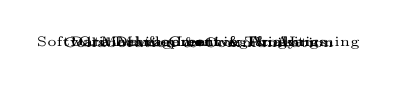
\begin{tikzpicture}[scale=1]
        \path   (0:0cm) coordinate (O);
        \foreach \X in {1,...,\D} {
            \draw (\X*\AG:0) -- (\X*\AG:\R);
        }
        \foreach \Y in {0,...,\U} {
            \foreach \X in {1,...,\D} {
                \path (\X*\AG:\Y*\R/\U) coordinate (D\X-\Y);
                \fill (D\X-\Y) circle (1pt);
            }
            \draw [opacity=0.3] (0:\Y*\R/\U) \foreach \X in {1,...,\D} {
                -- (\X*\AG:\Y*\R/\U)
            } -- cycle;
        }

        \path (1*\AG:\L*1.2) node (L1) {\tiny Software Development \& Programming};
        \path (2*\AG:\L*1.2) node (L2) {\tiny Data Management \& Analytics};
        \path (3*\AG:\L*1.2) node (L3) {\tiny Machine Learning \& AI};
        \path (4*\AG:\L*1.2) node (L4) {\tiny Critical \& Creative Thinking};
        \path (5*\AG:\L*1.2) node (L5) {\tiny Collaboration \& Communication};

        % AI eval
        \draw [color=red,line width=1.5pt,opacity=0.5]
            (D1-3) --
            (D2-3) --
            (D3-3) --
            (D4-3) --
            (D5-3) -- cycle;
        
        % Student re-eval
        \draw [color=blue,line width=1.5pt,opacity=0.5]
            (D1-3) --
            (D2-2) --
            (D3-3) --
            (D4-2) --
            (D5-3) -- cycle;

    \end{tikzpicture}
    \caption{Evaluation Radar Chart}
    \label{fig:eval-radar}
\end{figure}

From figure \ref{fig:eval-radar}, the red line represents the evaluated scores from the AI, the blue like represents the re-evaluation of students and the green line
represents the final evaluation by the advisor after peer reviewing.

% TODO: Add summary